\documentclass{jarticle}

\usepackage{graphicx}
\usepackage{url}
\usepackage{listings,jlisting}
\usepackage{ascmac}
\usepackage{amsmath,amssymb}

%ここからソースコードの表示に関する設定
\lstset{
  basicstyle={\ttfamily},
  identifierstyle={\small},
  commentstyle={\smallitshape},
  keywordstyle={\small\bfseries},
  ndkeywordstyle={\small},
  stringstyle={\small\ttfamily},
  frame={tb},
  breaklines=true,
  columns=[l]{fullflexible},
  numbers=left,
  xrightmargin=0zw,
  xleftmargin=3zw,
  numberstyle={\scriptsize},
  stepnumber=1,
  numbersep=1zw,
  lineskip=-0.5ex
}
%ここまでソースコードの表示に関する設定

\title{知能プログラミング演習II 課題1}
\author{グループ07\\
  29114007 池口 弘尚\\
%  {\small (グループレポートの場合は、グループ名および全員の学生番号と氏名が必要)}
}
\date{2019年10月7日}

\begin{document}
\maketitle

\paragraph{提出物} rep1
\paragraph{グループ} グループ07
\paragraph{メンバー}
\begin{tabular}{|c|c|c|}
  \hline
  学生番号&氏名&貢献度比率\\
  \hline\hline
  29114007&池口弘尚&0\\
  \hline
  29114031&大原拓人&0\\
  \hline
  29114048&北原太一&0\\
  \hline
  29114086&飛世裕貴&0\\
  \hline
  29114095&野竹浩二朗&0\\
\end{tabular}

\section{課題の説明}
\begin{description}
\item[課題1-1] Search.javaの状態空間におけるパラメータ(コストや評価値)を様々に変化させて実行し,
  各探索手法の違いを説明せよ.
  具体的には,変化させたパラメータと探索結果(最短パス探索の成否,
  解を返すまでのステップ数,etc.)の関係を,探索手法毎に表やグラフ等にまとめよ.
  それらの結果を参照して考察を行い,各探索手法の違いを説明せよ.
\item[課題1-2] グループでの進捗管理や成果物共有などについて,工夫した点や使ったツールについて考察せよ.
\item[課題1-3] Search.javaの探索過程や最終的に得られた順路をユーザに視覚的に示すGUIを作成せよ.
\end{description}


\section{課題1-1}
\begin{screen}
  Search.javaの状態空間におけるパラメータ(コストや評価値)を様々に変化させて実行し,
  各探索手法の違いを説明せよ.
  具体的には,変化させたパラメータと探索結果(最短パス探索の成否,
  解を返すまでのステップ数,etc.)の関係を,探索手法毎に表やグラフ等にまとめよ.
  それらの結果を参照して考察を行い,各探索手法の違いを説明せよ.
\end{screen}

課題 1-1 は実装を伴わない課題であるため、考察のみ記す。

\subsection{手法}
課題で与えられた探索手法は以下のとおりである。

\begin{enumerate}
\item 幅優先探索法
\item 深さ優先探索法
\item 分枝限定法
\item 山登り法
\item 最良優先探索法
\item A*アルゴリズム
\end{enumerate}


\subsection{考察}
幅優先探索では浅いノードから順に、そして深さ優先探索では深いノードから順に探索していくという手法である。ノードが有限であればどちらの探索法も全てのノードを探索するため、探索にかかる最悪時間に差はないといえる。しかし、深さ優先探索では先端までいきつくまで探索に失敗して戻ってっ来ることができないため、ノードが無限にあった場合探索終了しないことがある。コストなどを見ていないため、最適であるかの保証はどちらにもない。また、幅優先探索ではそれぞれの深さのノードをすべてオープンリストに入れなければならないため、深さが増えるごとにオープンリストのサイズが急激に増加することが考えられる。

つまり、これらの探索方法はそのままでは役に立つ場面が少ないと思われる。


\section{課題1-2}
\begin{screen}
  グループでの進捗管理や成果物共有などについて,工夫した点や使ったツールについて考察せよ.
\end{screen}

課題1-2は実装を伴わない課題であるため、考察のみ記す。

\subsection{考察}
今回は、扱っているデータがそれほど機密性の高いものではなかったため、連絡の手段としてはより気軽に使えることを重視して、LINEを使用した。

\section{課題1-3}
\begin{screen}
  Search.javaの探索過程や最終的に得られた順路をユーザに視覚的に示すGUIを作成せよ.
\end{screen}

発展問題に関しては、私が担当した。

\subsection{実装}
まず、新たに追加したクラスは以下の
\begin{itemize}
\item DrawArrowクラス: Path2D.Floatを継承。向きがある矢印の描画をするためのクラスであり、参考文献のコードを利用した。
\item FrameBaseクラス: JFrameを継承。コンストラクタのみ実装しており、JFrameの各種設定が1行でできるようにしてある。
\item GraphPanelクラス: JPanelを継承。各種グラフを描画するためのメソッドが実装されている。
\item MakeGUIクラス: 各種GUIを作成するためのクラス。
\end{itemize}

DrawArrowクラスについては参考文献\cite{goo}をそのまま用いた。

FrameBaseクラスでは、JFrameのサイズやウィンドウを閉じたときにプログラムを終了することなどを一括して設定するためのコンストラクタを以下のように実装した。

\begin{lstlisting}[caption=FrameBaseのコンストラクタ,label=src:FrameBase]
	//位置を指定
    public FrameBase(String title,int x,int y,int width,int height) {
		setTitle(title);
		setBounds(x, y, width, height);
		setDefaultCloseOperation(JFrame.EXIT_ON_CLOSE);
	}
	//中央に表示
	public FrameBase(String title,int width,int height) {
		setTitle(title);
		setSize(width, height);
		setLocationRelativeTo(null);
		setDefaultCloseOperation(JFrame.EXIT_ON_CLOSE);
	}
\end{lstlisting}

GraphPanelクラスでは、探索のグラフを表示するための様々なメソッドが実装してある。
探索木を表示することに関連するmakeTreeList,addTreeList,selectTreeNode,
removeNodeFromTree,addLeaf,addGoalは以下のように実装した。
\begin{lstlisting}[caption=探索木関連のメソッド,label=src:MakeGUI1]
	//ルートノードを作成
	public void makeTreeList(Node root) {
		nodeMap = new HashMap<>();
		//clear();
		DefaultMutableTreeNode rootNode = new DefaultMutableTreeNode(root);
		nodeMap.put(root.name, rootNode);
		tree = new JTree(rootNode);
		add(tree);
		setVisible(false);
		setVisible(true);
	}
	//pをcの親にする
	public void addTreeList(Node p, Node c) {
		DefaultMutableTreeNode parent = nodeMap.get(p.name);
		if (parent == null) {
			System.out.println("error");
			return;
		}
		DefaultMutableTreeNode child = new DefaultMutableTreeNode(c);
		parent.add(child);
		nodeMap.put(c.name, child);
		DefaultTreeModel m = (DefaultTreeModel) tree.getModel();
		m.reload();
		for (int i = 0; i < tree.getRowCount(); i++) {
			tree.expandRow(i);
		}
	}
	
    //nodeを選択状態にする
	public void selectTreeNode(Node node) {
		DefaultMutableTreeNode p = nodeMap.get(node.name);
		tree.setSelectionPath(new TreePath(p.getPath()));
	}

	//cをルートとする木を親ノードから除く
	public void removeNodeFromTree(Node c) {
		DefaultMutableTreeNode child = nodeMap.get(c.name);
		if (child != null) {
			child.removeFromParent();
		}
	}

	//pにリーフノードをつける
	public void addLeaf(Node p) {
		DefaultMutableTreeNode parent = nodeMap.get(p.name);
		if (parent == null) {
			System.out.println("error");
			return;
		}
		parent.add(new DefaultMutableTreeNode("leaf"));
		DefaultTreeModel m = (DefaultTreeModel) tree.getModel();
		m.reload();
		for (int i = 0; i < tree.getRowCount(); i++) {
			tree.expandRow(i);
		}
	}

	//pにgoalノードをつける
	public void addGoal(Node p) {
		DefaultMutableTreeNode parent = nodeMap.get(p.name);
		if (parent == null) {
			System.out.println("error");
			return;
		}
		parent.add(new DefaultMutableTreeNode("Goal"));
		DefaultTreeModel m = (DefaultTreeModel) tree.getModel();
		m.reload();
		for (int i = 0; i < tree.getRowCount(); i++) {
			tree.expandRow(i);
		}
	}
\end{lstlisting}

また、局所的な解法に関連するメソッドmakeLocalGraphは以下のように実装した。
\begin{lstlisting}[caption=makeLocalGraph,label=src:MakeGUI2]
	public void makeLocalGraph(Node root) {
		setLayout(null);
		removeAll();
		JLabel rootlab = makeNodeLabel(root,Color.RED, 150, 200);
		int num = root.getChildren().size();
		if (num == 1) {
			JLabel child = makeNodeLabel(root.getChildren().get(0),Color.BLUE, 700, 200);
			add(child);
		} else {
			int t = 400/(num-1);
			for (int i = 0; i < num; i++) {
				JLabel child = makeNodeLabel(root.getChildren().get(i),Color.BLUE, 700, t*i);
				add(child);
			}
		}
		add(rootlab);
		setVisible(false);
		setVisible(true);
	}
\end{lstlisting}

上記のGraphPanelを利用して、必要なGUIを作成するクラスMakeGUIは以下のように実装した。
\begin{lstlisting}[caption=MakeGUI,label=src:MakeGUI3]
public class MakeGUI {

	public static void MakeChooseSearchGUI(ActionListener listener, String[] searchNames) {
		FrameBase frame = new FrameBase("test", 500, 500);
		JPanel panel = new JPanel();
		for (int i = 0; i < searchNames.length; i++) {
			JButton but = new JButton(searchNames[i]);
			but.addActionListener(listener);
			but.setActionCommand(searchNames[i]);
			panel.add(but);
		}
		panel.setLayout(new GridLayout(searchNames.length, 1));
		frame.getContentPane().add(panel);
		frame.setVisible(true);
	}

	public static GraphPanel MakeSearchGUI(ActionListener listener) {
		FrameBase frame = new FrameBase("test", 1000, 500);
		GraphPanel gPanel = new GraphPanel(1000, 500);
		JPanel p = new JPanel();
		JButton btn1 = new JButton("閉じる");
		btn1.addActionListener(listener);
		btn1.setActionCommand("close");
		JButton btn2 = new JButton("1ステップ");
		btn2.addActionListener(listener);
		btn2.setActionCommand("step");
		JButton btn3 = new JButton("最後まで");
		btn3.addActionListener(listener);
		btn3.setActionCommand("last");

		p.add(btn1);
		p.add(btn2);
		p.add(btn3);

		JPanel p2 = new JPanel();
		JLabel label1 = new JLabel("Step:");
		JLabel label2 = new JLabel();
		p2.add(label1);
		p2.add(label2);
		gPanel.SetStepLabel(label2);

		frame.getContentPane().add(p2, BorderLayout.NORTH);
		frame.getContentPane().add(p, BorderLayout.SOUTH);
		frame.getContentPane().add(gPanel, BorderLayout.CENTER);
		frame.pack();
		frame.setVisible(true);

		return gPanel;
	}
}
\end{lstlisting}

\subsection{実行例}
実行すると次のようなGUIが表示される。


\begin{figure}[!hbt]
  \centering
  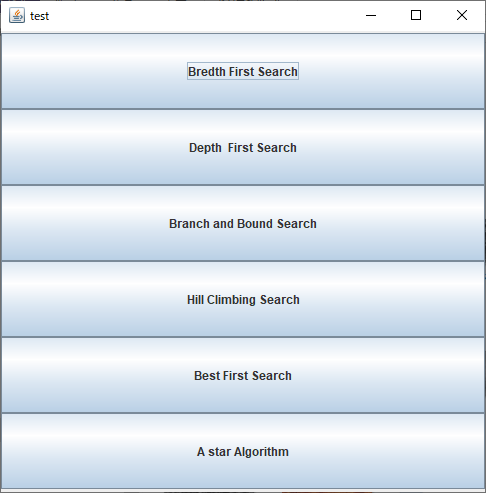
\includegraphics[bb=0 0 487 493,width=0.6\linewidth]{gui1.png}
  \caption{探索方法の選択}
  \label{fig:gui1}
\end{figure}

この中から行いたい探索方法を選んでクリックする。探索が終わると次のようになる。


\begin{figure}[!hbt]
  \centering
  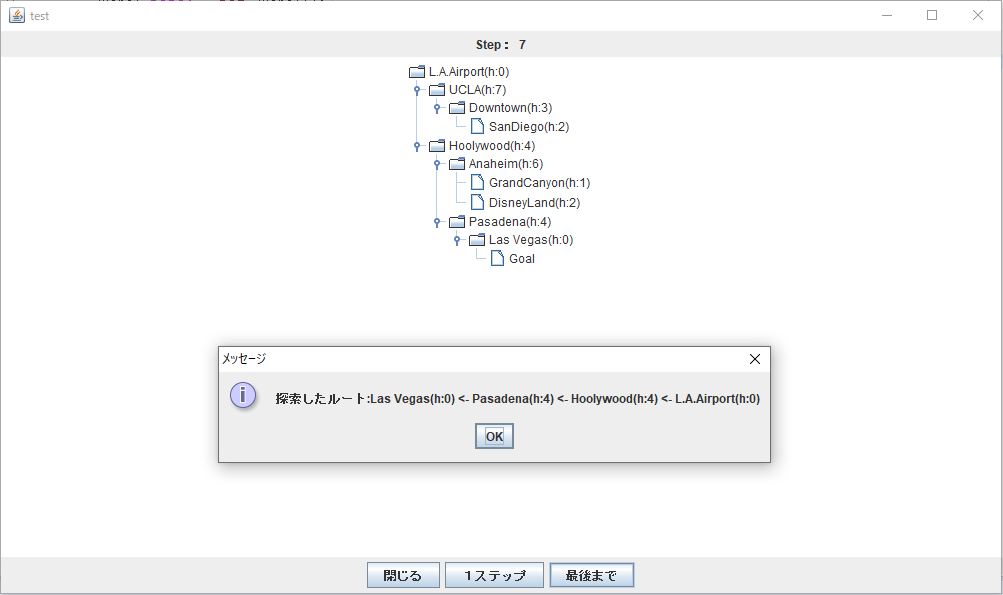
\includegraphics[bb=0 0 1003 595,width=1\linewidth]{gui2.png}
  \caption{探索終了}
  \label{fig:gui2}
\end{figure}
\subsection{考察}
今回の実装ではswingを使用してGUIを作成した。swingには、ウィンドウや各種のボタンなどは取り揃えてあった。
しかし、元々描画をするためのものではないようなので、図形を描画したり、レイアウトの位置を座標で指定したいときには新しいクラスを作った方が良いと考えられる。この実装では、レイアウトの方が間に合わなかったため、探索木はJTreeを利用した。

今回作ったGUIでは、1ステップごとに状況を確認できるように1ステップごとに進む機能が実装されている。
この実装ではビジーウェイトなどを使わないようにするため、スレッドを分けてwaitとnotifyで実現している。それらは以下のように実装した。
\begin{lstlisting}[caption=wait部分,label=src:wait]
synchronized public void breadthFirst() {
        ...
        for (;;) {
            //1ステップごとに進むかどうか
            if (isStop) {
                try {
                    wait();
                } catch (InterruptedException e) {
                    // TODO 自動生成された catch ブロック
                    e.printStackTrace();
                }
            }
        ...
    }
\end{lstlisting}

\begin{lstlisting}[caption=notify部分,label=src:notify]
    ActionListener listener = new ActionListener() {

        //ボタンを押したときに呼ばれるメソッド
        @Override
        public void actionPerformed(ActionEvent e) {
            String cmd1 = e.getActionCommand();
            switch (cmd1) {
            //プログラムを終了する
            case "close":
                System.exit(0);
                break;
            //1ステップ進む
            case "step":
                synchronized (sh) {
                    sh.notifyAll();
                }
                break;
            //最後まで進む
            case "last":
                sh.isStop = false;
                synchronized (sh) {
                    sh.notifyAll();
                }
                break;
            default:
                break;
            }
        }
    };
\end{lstlisting}

waitやnotifyはObjectに対して働くため、Runnnableを作ってそこにSearchのメソッドを入れるという方法ではうまくいかなかった。
これはSearchのインスタンスとRunnnableのインスタンスが別であったために生じたことであると考えられる。
これを解決するため、SearchにRunnnableをimplementし、それをThreadの中に入れることによって、この問題を解決することができた。

\section{感想}



% 参考文献
\begin{thebibliography}{99}
\bibitem{goo} 矢印を描画 -JAVAで矢印を描画したいのですが、どうしたらいいのかわか- Java | 教えて!goo
\url{https://oshiete.goo.ne.jp/qa/4014364.html} (2019年10月7日アクセス).
\bibitem{swing} Swingを使ってみよう - Java GUIプログラミング
\url{https://www.javadrive.jp/tutorial/} (2019年10月7日アクセス).

%\bibitem{hanako} 工大花子さんのレポート。また、・・・を教えてもらった 

\end{thebibliography}

\end{document}
